\subsection{Barycentric coordinates}\label{section:barycentric-coord}
Barycentric coordinates, discovered by M\"obius in 1827, represent one of the most progessive area of research in computer graphics and mathematics thanks to the numerous applications in image and geometry processing.
\cite{REPORT:localbarycentricoordsepfl}
% ------
The position of any point in a triangle can be expressed using a linear combination of barycentric coordinates:
$$ p = \lambda_1 p_1 + \lambda_2 p_2 + \lambda_3 p_3$$
where $p_1$, $p_2$ and $p_3$ are the vertices of a triangle and $\lambda_1$, $\lambda_2$ and $\lambda_3$ (the barycentric coordinates) are three scalars that
respect the following barycentric coordinates properties.\cite{SLIDE:ICORSI}
% -------
\begin{itemize}
  \item partition of unity: $\sum_{i=1}^3 \lambda_{i}(p) = 1$
  \item reproduction: $\sum_{i=1}^3 \lambda_{i}(p)p_i = p$
  \item Lagrange-property: $\lambda_i(p_j) = \delta_{i, j}$
  \item linearity: $\lambda_i \in \prod_1$
  \item non-negativity: $\lambda_i(p)\geq 0$ for $p \in [p_1, p_2, p_3]$
\end{itemize}

% -------
A point is inside the triangle if and only if $0 \leq \lambda_1, \lambda_2, \lambda_3 \leq 1$. If a barycentric coordinate is less than zero or greater than one, the point is outside the triangle.
% -------
Barycentric coordinates allow the interpolation of values, from a set of control points over the interior of a domain, using weighted combinations of values associated with the control points (Fig. \ref{fig:barycentric-coord}).
\cite{REPORT:localbarycentricoordsepfl}
% ------
\begin{figure}[h!]
  \centering
  \scalebox{.7}{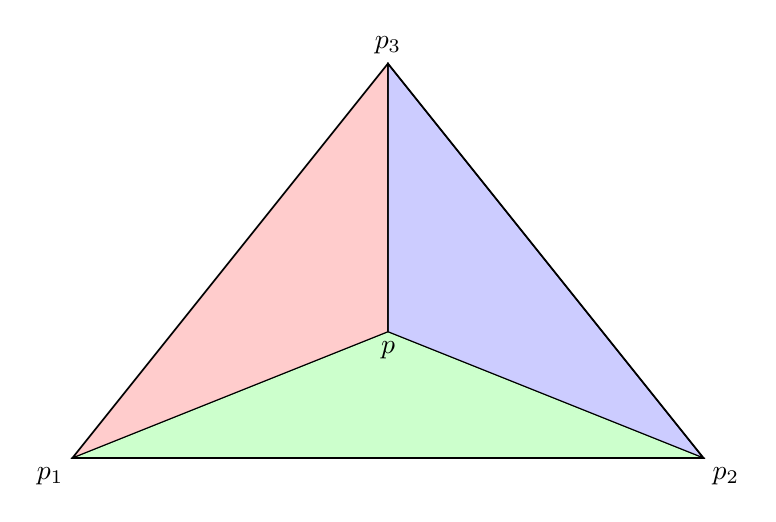
\begin{tikzpicture}
    \coordinate (L1) at (0,0);
    \coordinate (L2) at (8,0);
    \coordinate (L3) at (4,5);
    \coordinate (X) at (4,1.6);

    \draw[thick] (L1) -- coordinate[midway](md3) (L2)
                      -- coordinate[midway](md1) (L3)
                      -- coordinate[midway](md2) (L1) -- cycle;
    \filldraw[draw=black, fill=green!20] (L1) -- (X) -- (L2) -- cycle;
    \filldraw[draw=black, fill=red!20] (L1) -- (X) -- (L3) -- cycle;
    \filldraw[draw=black, fill=blue!20] (L3) -- (X) -- (L2) -- cycle;
    \draw (L1) node [below left] {$p_1$}
       -- (L2) node [below right] {$p_2$}
       -- (L3) node [above] {$p_3$}
       -- (X) node [below] {$p$};
    \end{tikzpicture}}
    \caption{Let $w_1$ be the blue area, $w_2$ the red one and $w_3$ the green one. Normalizing each of them by the area of the triangle will return three values ($\lambda_1, \lambda_2, \lambda_3$) that are the barycentric coordinates of $p$ with respect to the triangle [$p_1, p_2, p_3$].}
    \label{fig:barycentric-coord}
  \end{figure}

%%%%%%%%%%%%%%%%%%%%%%%%%%%%%%%%%%%%%%%%%%%%%%%%%%%%%%%%%%%%%%%%%

\subsection{Triangle meshes}
A collection of triangles without any particular mathematical structure is called \textit{triangle meshes}. To derive a global parameterization for an entire triangle mesh we can define a 2D position for each vertex. Let $\mathcal{M}$ be a triangle mesh that consists of a geometric and topological component represented by a graph structure with a set of vertices $\mathcal{V} = \{ v_1, ..., v_V \}$ and a set of triangular faces connecting them $\mathcal{F} = \{ f_1, ... , f_F \}$ with $f_i \in \mathcal{V} \times \mathcal{V} \times \mathcal{V}$. The connectivity of a triangle mesh can be expressed in termes of the edges of the respective graph $\mathcal{E} = \{ e_1, ..., e_E \}$ where $e_i \in \mathcal{V} \times \mathcal{V}$.
\cite{polygonmeshprocessing}
\begin{figure}[h!]
  \centering
  \minipage[b]{.5\linewidth}
  \includegraphics[scale=0.2]{images/armadillo-white04}
  \endminipage
  \minipage[b]{.5\linewidth}
  \includegraphics[scale=0.2]{images/armadillo-white205}
  \endminipage
\caption{3D triangle meshes.}

\end{figure}

%%%%%%%%%%%%%%%%%%%%%%%%%%%%%%%%%%%%%%%%%%%%%%%%%%%%%%%%%%%%%%%%%

\subsection{Lighting - Phong lighting model}

\begin{figure}[h!]
  \centering
  \includegraphics[scale=0.6]{images/lighting}
\caption{Lighting notation for Phong lighting model. \cite{SLIDE:ICORSI}}
\end{figure}
Given a light source at position $l$ with intensity $I_l$ and a surface point at position $p$ with normal $n$,
we can define the angle between the incident light ($l-p$) and the normal $n$ as $\varphi$.
Let $r$ be our reflected light vector defined as $r = 2 n \cdot <n, l - p> - (l-p)$ and $\alpha$ the angle between that vector and the view direction $(v - p)$.

The \textit{Phong lighting model} is defined as the sum of the self-emitting intensity, ambient term, diffuse reflection and specular reflection.
$$ I = I_e + {\rho}_a \cdot I_A + \sum_{j=1}^n ({\rho}_d \cdot cos {\varphi}_j + {\rho}_s \cdot cos_{\alpha_j}^k) \cdot I_j$$ where $I_e$ is the self-emitting intensity, ${\rho}_a, {\rho}_d, {\rho}_s$ are the reflection constants (surface properties), $n$ is the number of lights sources with intensities $I_j$ and $k$ is the shininess.
\cite{SLIDE:ICORSI}

%%%%%%%%%%%%%%%%%%%%%%%%%%%%%%%%%%%%%%%%%%%%%%%%%%%%%%%%%%%%%%%%%

\subsection{Linear interpolation}\label{section:linear-interpolation}
Linear interpolation is a method that will return equal spacing between the interpolated values. Given two numbers $n_1$ and $n_2$ (the start and final values of the interpolant), a linear interpolation can be carried out using a parameter $t$ ($t \in [0,1]$). \cite{WEBSITE:interpolation}

$$ n = n_1 + t (n_2 - n_1)$$


The standard linear interpolated visualization is made passing three attributes (colors) to each vertex of a triangle. OpenGL will interpolate these colors linearly thanks to the barycentric coordinates that will tell how much of each color is being mixed at any position.
Given a triangle $[p_1, p_2, p_3]$, where the color blue is passed to vertex $p_1$, red to $p_2$, and green to $p_3$, let be $w_1$ the blue area, $w_2$ the red area and $w_3$ the green area (See Fig. \ref{fig:barycentric-coord}). Let us define the value at $p$ as a \textit{barycentric interpolation} $$(w_1p_1 + w_2p_2 + w_3p_3)/W$$ where $W$ is the area of the triangle $[p_1, p_2, p_3]$.

%%%%%%%%%%%%%%%%%%%%%%%%%%%%%%%%%%%%%%%%%%%%%%%%%%%%%%%%%%%%%%%%%

\subsection{Flat Shading}
\textit{Flat shading} is a way to compute the color at each pixel (at a corner or at the barycentre) using the triangle normal.
Given a triangle $[p_1, p_2, p_3]$, the lighting is computed using the normal $n$ $$\widehat{n} = (p_2 - p_1) \times (p_3 - p_1) \;\;\;\;\;\;\;\; n = \frac{ \widehat{n} } { ||\widehat{n}|| } $$ at $p= (p_1 + p_2 + p_3)/3$. This color is then used for all pixels. Flat shading gives objects with flat facets.
\cite{SLIDE:ICORSI}
%%%%%%%%%%%%%%%%%%%%%%%%%%%%%%%%%%%%%%%%%%%%%%%%%%%%%%%%%%%%%%%%%

\subsection{Gouraud Shading}
\textit{Gouraud Shading} is a way to compute the color at each pixel assigning a normal to each corner of a triangle and after having computed the color for each corner it linearly interpolates these color values (see Sections \ref{section:barycentric-coord} and \ref{section:linear-interpolation}).
Given a triangle $[p_1, p_2, p_3]$ and the normal at each corner $n_1, n_2, n_3$, the lighting is computed at $p_i$ using the normal $n_i$. This process applied to each corner returns the color values $c_1, c_2, c_3$ respectively for $p_1, p_2$ and $p_3$.
These colors are then linearly interpolate $c = {\mu}_1 c_1 + {\mu}_2 c_2 + {\mu}_3 c_3$. Gouraud shading gives objects that appear more smooth. \cite{SLIDE:ICORSI}

%%%%%%%%%%%%%%%%%%%%%%%%%%%%%%%%%%%%%%%%%%%%%%%%%%%%%%%%%%%%%%%%%


